\documentclass[12pt]{kiarticle} % You can learn about my document class "kiarticle" and install it to your device by following the link: https://github.com/Kiarendil/toolkitex
\graphicspath{{pictures/}}
\DeclareGraphicsExtensions{.pdf,.png,.jpg,.eps}
%%%
\pagestyle{fancy}
\fancyhf{}
%\renewcommand{\headrulewidth}{ 0.1mm }
\renewcommand{\footrulewidth}{ .0em }
\fancyfoot[C]{\texttt{\textemdash~\thepage~\textemdash}}
\fancyhead[L]{Лабораторная работа № 4.4.4 \hfil}
\fancyhead[R]{\hfil Иванов Кирилл, 625 группа }
\usepackage{multirow} % Слияние строк в таблице
\newcommand
{\un}[1]
{\ensuremath{\text{#1}}}
\newcommand{\eds}{\ensuremath{ \mathscr{E}}}
\usepackage{tikz}
%%% Работа с таблицами
\usepackage{array,tabularx,tabulary,booktabs} % Дополнительная работа с таблицами
\usepackage{longtable}  % Длинные таблицы
\usepackage{multirow} % Слияние строк в таблице

\begin{document}
	
	\begin{titlepage}
	\begin{center}
		\large 	Московский физико-технический институт \\
		(государственный университет) \\
		Факультет общей и прикладной физики \\
		\vspace{0.2cm}
		
		\vspace{4.5cm}
		Лабораторная работа № 4.4.4 \\ \vspace{0.2cm}
		\large (Общая физика: оптика) \\ \vspace{0.2cm}
		\LARGE \textbf{Интерферометр Фабри-Перо}
	\end{center}
	\vspace{2.3cm} \large
	
	\begin{center}
		Работу выполнил: \\
		Иванов Кирилл,
		625 группа
		\vspace{10mm}		
		
	\end{center}
	
	\begin{center} \vspace{60mm}
		г. Долгопрудный \\
		2018 год
	\end{center}
\end{titlepage}
	
	\paragraph*{Цель работы:} 
	
	\paragraph*{Оборудование:} 
	
	\section{Экспериментальная установка}
	
	Схема экспериментальной установки представлена на рис. 1. Свет от ртутной лампы $ S $, пройдя через линзу $ Л_0 $ и светофильтр $ C $, попадает на интерферометр Фабри-Перо (ИФП). Линза $ Л_0 $ служит для
	формирования пучка лучей (слегка сходящегося или слегка расходящегося). Интерференционные кольца наблюдаются в локальной плоскости линзы $ Л $. Картина рассматривается через зрительную трубу $ Т $, сфокусированную на эту плоскость. Диаметры колец измеряются с помощью микроскопа катетометра.
	
		\begin{figure}[h!]
		\centering
		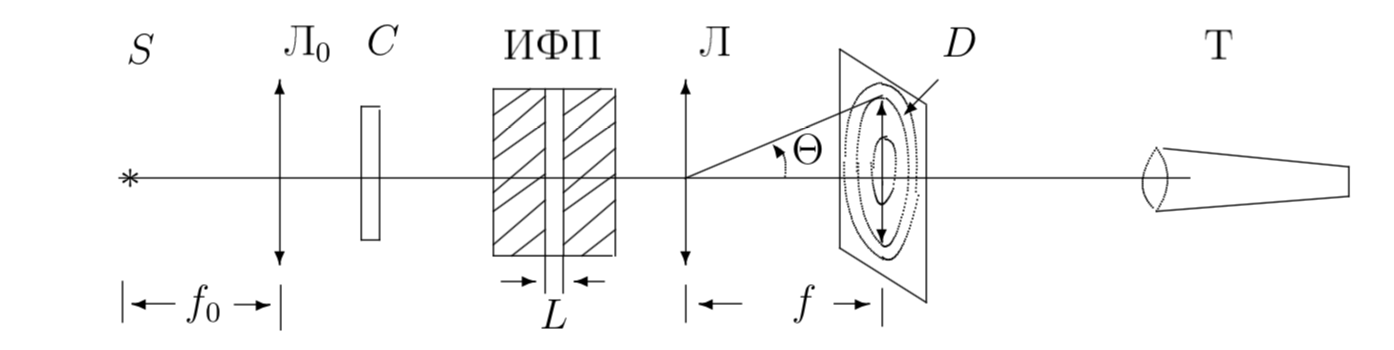
\includegraphics[width=\linewidth]{lab.png}
		\caption{Экспериментальная установка}
		\label{lab}
	\end{figure}

	
	Зрительная труба $ Т $ и отсчетный микроскоп  --- элементы катетометра --- прибора, предназначенного для измерения расстояний в вертикальной плоскости вдоль вертикальной оси. 
	При достаточной яркости ртутной лампы можно увидеть, что зелёная линия
	ртути состоит из нескольких компонентов. Расщепление этой спектральной линии связано с дополнительной энергией, возникающей как в результате взаимодействия магнитных моментов ядра и электрона --- \textit{сверхтонкая структура} (магнитное поле ядра действует на спиновый магнитный момент электрона), так и с \textit{изотопическим сдвигом} (в парах ртути присутствуют в заметных количествах изотопы с атомными массами от 198 до 204 а.е.м.). Каждое зелёное кольцо содержит более десятка близко расположенных компонентов, но разрешение нашего прибора не позволяет все их рассмотреть.
	Спектр натриевой лампы исследуется по аналогичной схеме, но светофильтр в этом случае не нужен, а интерферометр, линзы и зрительная труба катетометра
	имеют другие параметры.
	
		\section{Ход работы}
		
		\subsection{Ртутная лампа}
		
		После настройки интерферометра проведем измерения диаметров зеленых и желтых интерференционных колец с помощью катетометра, оценивая его погрешность измерения как $ \sigma_l = 0,3 $ мм. Параметр установки --- фокусное расстояние линзы $ f = 110 $ мм.
		
		Будем последовательно измерять расстояния $ l_1 $ от верхнего края 6-ого "<набора"> колец до нуля до центра, затем аналогично будем измерять расстояния $ l_2 $ от нижнего края до нуля. Результаты занесем в таблицы. 
		
			\begin{table}[]
			\caption{Измерение диаметров зеленых колец ртутной лампы}
			\begin{center}
				\begin{tabular}{|c|c|c|c|c|}
					\hline
					$ N $ & $ l_1 $, мм & $ l_2 $, мм & $ d_i^2 $, $ мм^2 $ & $ \sigma_d $, мм\\
					\hline
					 1 & 167.61 & 179.85 & 1.5 & 0.01 \\
					2 & 163.87 & 183.55 & 3.88 & 0.03 \\
					3 & 161.19 & 186.11 & 6.21 & 0.05 \\
					4 & 159.16 & 188.15 & 8.4 & 0.07 \\
					5 & 157.39 & 189.96 & 10.61 & 0.09 \\
					6 & 155.82 & 191.55 & 12.77 & 0.11 \\
					\hline
				\end{tabular}
			\end{center}
			\label{Gr_table}
		\end{table}
	
	\begin{table}[]
		\caption{Измерение диаметров желтых колец ртутной лампы}
		\begin{center}
			\begin{tabular}{|c|c|c|c|c|c|c|c|c|}
				\hline
					$ N $ & $ l_1 $, мм & $ l_2 $, мм & $ d $, мм & $ \overline{d} $,мм &  $ \sigma_d $,мм & $ \Delta d $, мм  &  $ 1/\Delta d $,$ мм^{-1} $ & $ \sigma_{1/\Delta d} $,$ мм^{-1} $\\
					\hline
			1 & 170.38 & 176.93 & 6.55 & 6.55 & 0.42 & 0 & - & - \\
			2 & 166.66 & 180.88 & 14.22 & 15.78 & 0.42 & 3.12 & 0.32 & 0.04 \\
			\text{} & 164.94 & 182.275 & 17.33 & \text{} & \text{} & \text{} & \text{} & \text{} \\
			
			3 & 162.94 & 184.27 & 21.33 & 22.31 & 0.42 & 1.97 & 0.51 & 0.08 \\
			\text{} & 161.995 & 185.295 & 23.3 & \text{} & \text{} & \text{} & \text{} & \text{} \\
			4 & 160.53 & 186.85 & 26.315 & 27.15 & 0.42 & 1.68 & 0.6 & 0.12 \\
			\text{} & 159.7 & 187.69 & 27.99 & \text{} & \text{} & \text{} & \text{} & \text{} \\
			5 & 158.36 & 188.95 & 30.585 & 30.96 & 0.42 & 1.35 & 0.74 & 0.18 \\
			\text{} & 157.69 & 189.03 & 31.34 & \text{} & \text{} & \text{} & \text{} & \text{} \\
			6 & 156.62 & 190.66 & 34.045 & 34.61 & 0.42 & 1.11 & 0.9 & 0.24 \\
			\text{} & 156.09 & 191.24 & 35.155 & \text{} & \text{} & \text{} & \text{} & \text{} \\
				\hline
			\end{tabular}
		\end{center}
		\label{Ye_table}
	\end{table}

	При этом погрешность $ \sigma_{1/\Delta d} $мы оценивали как $ \sigma_{1/\Delta d} = \dfrac{\sigma_{\Delta d}}{\Delta d} \x \dfrac{1}{\Delta d} $.
	
	Построим графики для зеленых и желтых колец:
	
		\begin{figure}[h]
		\label{gr_graf}
		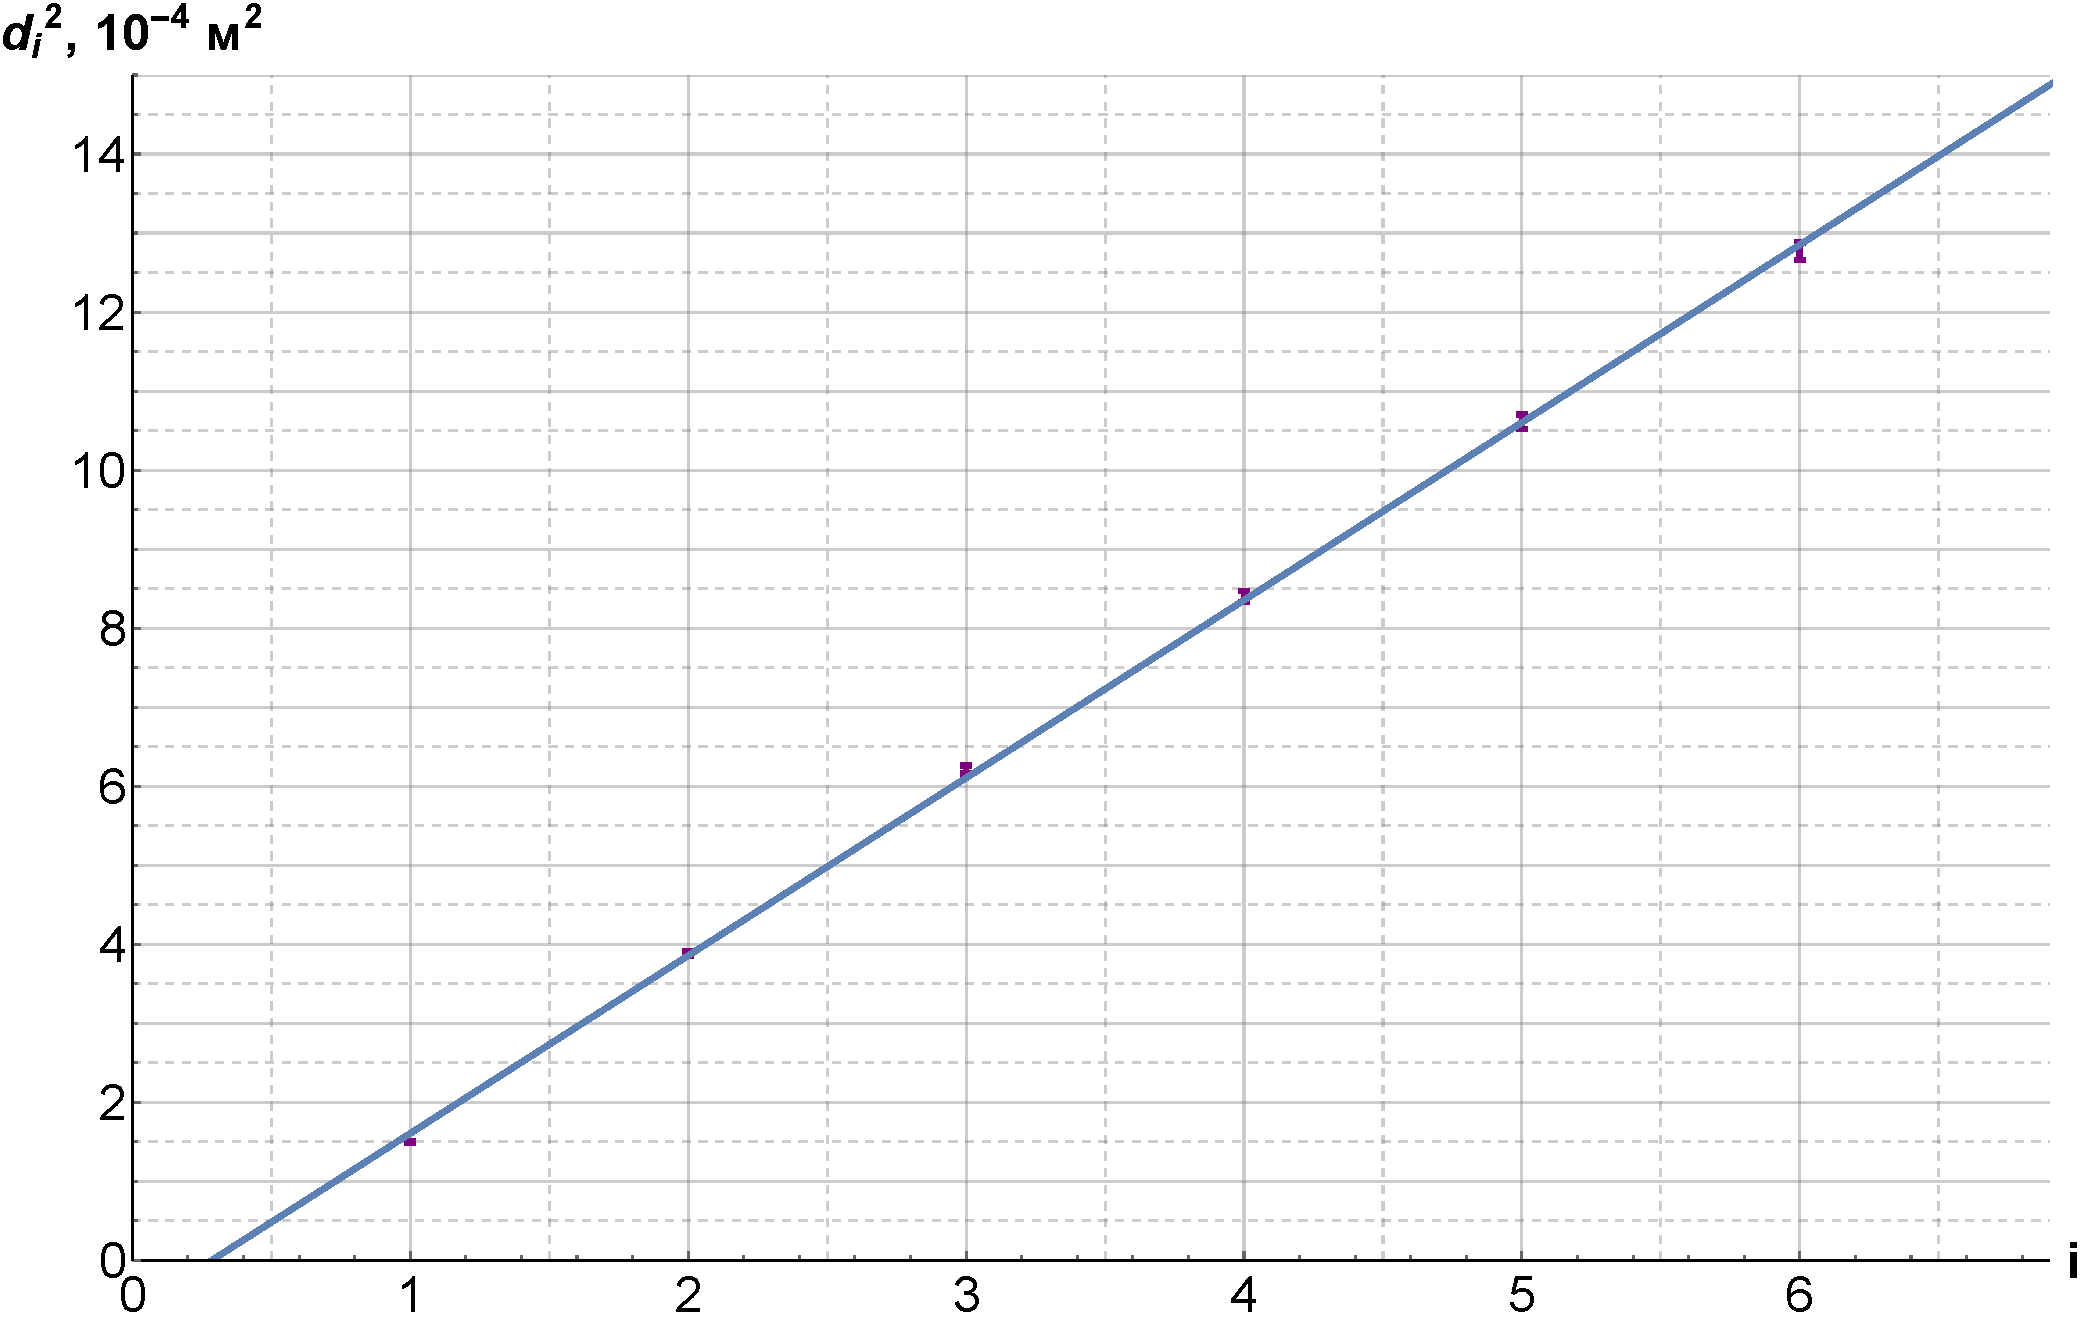
\includegraphics[scale=0.47]{green.pdf}
		\caption{График зависимости $ d_i^2 $ от $ i $ зеленых линий $ Hg $}
	\end{figure}
	
	\begin{table}[h]
		\centering
		\caption{Расчет апроксимированной прямой $ y = ax +b $}
		\begin{tabular}{c|cc}
			\text{} & \text{Estimate} & \text{Standard Error} \\
			\hline
			a & 
				2.25 & 0.02
			 \\
			b & -0,64 & 0.08  \\
		\end{tabular}
	\end{table}

	Из полученных данных $ a = \dfrac{\varDelta (d_i^2)}{  \varDelta(i) } = (2,25 \pm 0,02) \x 10^{-4} \; м^2 $ рассчитаем базу $ L $ интерферометра, взяв $ \lambda(Hg) =  5461 $ \AA :
	
	
	\begin{equation}\label{}
	\dfrac{\lambda}{L} = \dfrac{a}{4f^2}
	\te L = 0,117 \pm 0,001 \;мм 
	\end{equation}
	
	\begin{figure}[h]
		\label{ye_graf}
		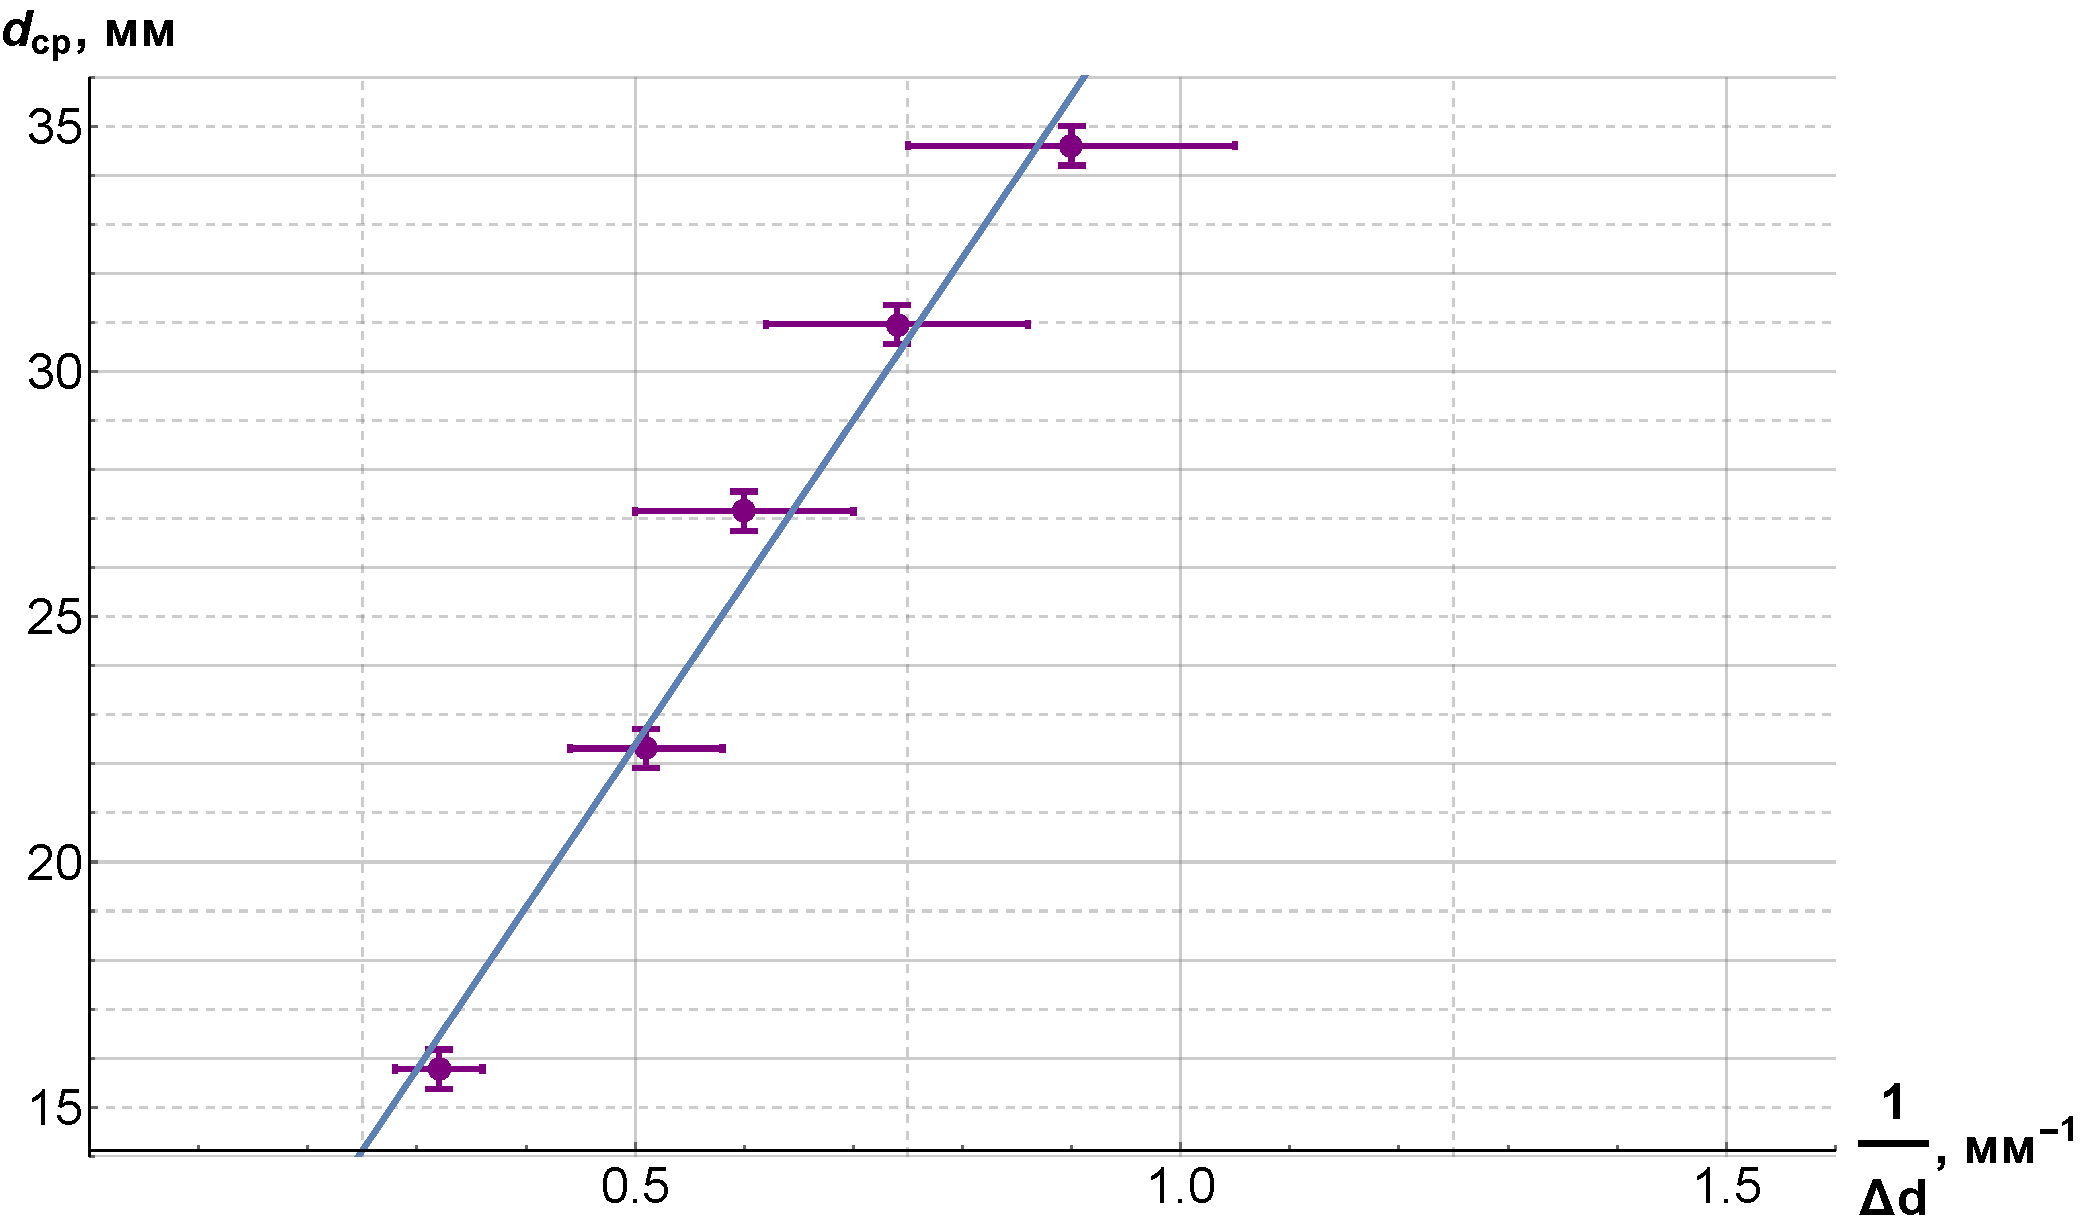
\includegraphics[scale=0.47]{yellow.pdf}
		\caption{График зависимости $ \overline{d} $ от $ \dfrac{1}{\Delta d}$ желтых линий $ Hg $}
	\end{figure}
	
	\begin{table}[h]
		\centering
		\caption{Расчет апроксимированной прямой $ y = ax +b $}
		\begin{tabular}{c|cc}
			\text{} & \text{Estimate} & \text{Standard Error} \\
			\hline
			a & 
			33,1 & 2,7
			\\
			b & 5,8 & 1,7  \\
		\end{tabular}
	\end{table}

	Из полученных данных $ a = \overline{d} \Delta d = (33,1 \pm 2,7) \x 10^{-6} м^2 $ рассчитаем разность длин волн $ \Delta \lambda_р  $ интерферометра, взяв $ \lambda(Hg) =  5780 $ \AA :
	
	\begin{equation}\label{}
	\Delta \lambda_р = \dfrac{\lambda a}{4f^2} = (3,9 \pm 0,3) \text{\AA}
	\end{equation}

	\subsection{Натриевая лампа}
	
	Проведем аналогичные измерения, сначала взяв одно из колец дублета ("<дальнее"> от центра), а затем для дублета. Фокусное расстояние $ f = 94 \; мм $. Результаты занесем в таблицу и построим графики.
	
	\begin{table}[]
		\caption{Измерение диаметров натриевых колец ртутной лампы}
		\begin{center}
			\begin{tabular}{|c|c|c|c|c|c|c|c|c|c|}
				\hline
				$ N $ & $ l_1 $, мм & $ l_2 $, мм & $ d $, мм  & $ d_i^2 $, $ мм^2 $ &$ \overline{d} $,мм &  $ \sigma_d $,мм & $ \Delta d $, мм  &  $ 1/\Delta d $,$ мм^{-1} $ & $ \sigma_{1/\Delta d} $,$ мм^{-1} $ \\
				\hline
				 1 & 148.89 & 140.49 & 8.4 & 0.71 & \text{--} & \text{} & - & \text{} & \text{} \\
				 2 & 152.29 & 137.27 & 15.03 & 2.26 & 16.14 & 0.59 & 2.22 & 0.45 & 0.05 \\
				 \text{} & 153.4 & 136.15 & 17.25 & \text{} & \text{} & \text{} & \text{} & \text{} & \text{} \\
				 3 & 155.29 & 134.13 & 21.16 & 4.48 & 21.97 & 0.59 & 1.61 & 0.62 & 0.07 \\
				 \text{} & 156.08 & 133.31 & 22.77 & \text{} & \text{} & \text{} & \text{} & \text{} & \text{} \\
				 4 & 157.62 & 131.77 & 25.85 & 6.68 & 26.46 & 0.59 & 1.22 & 0.82 & 0.09 \\
				 \text{} & 158.22 & 131.15 & 27.07 & \text{} & \text{} & \text{} & \text{} & \text{} & \text{} \\
				 5 & 159.61 & 129.85 & 29.76 & 8.86 & 30.33 & 0.59 & 1.13 & 0.88 & 0.12 \\
				 \text{} & 160.16 & 129.27 & 30.89 & \text{} & 0 & \text{} & \text{} & \text{} & \text{} \\
				 6 & 161.17 & 128.11 & 33.06 & 10.93 & 33.56 & 0.59 & 1.01 & 0.99 & 0.14 \\
				 \text{} & 161.71 & 127.65 & 34.07 & \text{} & \text{} & \text{} & \text{} & \text{} & \text{} \\
				\hline
			\end{tabular}
		\end{center}
		\label{Na2_table}
	\end{table}

	

	\begin{figure}[h]
		\label{na1_graf}
		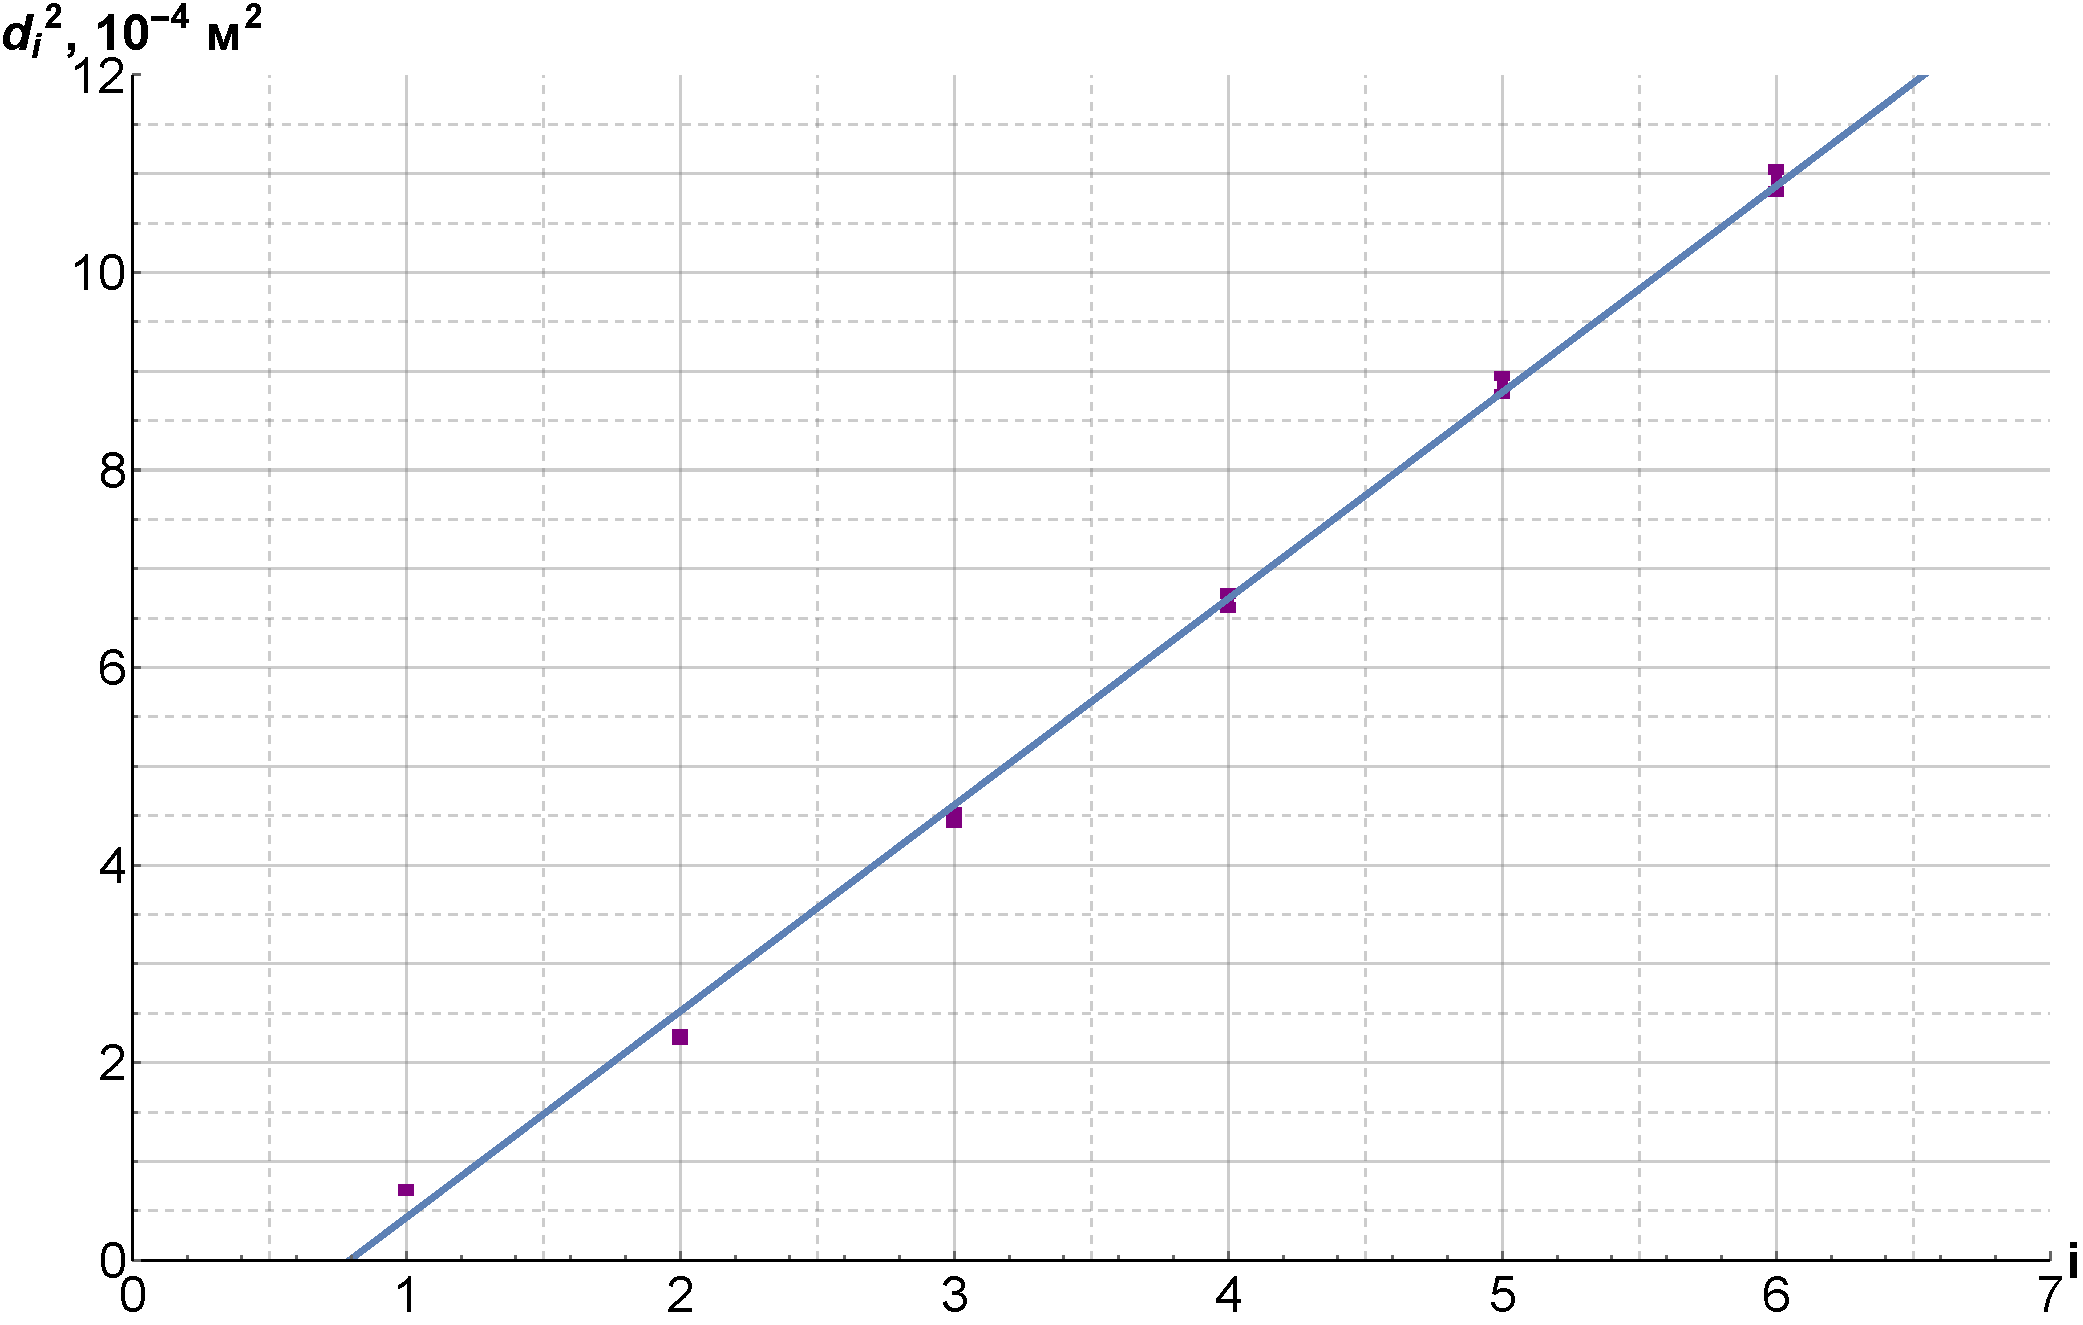
\includegraphics[scale=0.47]{na1.pdf}
		\caption{График зависимости $ d_i^2 $ от $ i $ одной из линии дублета $ Na $}
	\end{figure}
	
	\begin{table}[h]
		\centering
		\caption{Расчет апроксимированной прямой $ y = ax +b $}
		\begin{tabular}{c|cc}
			\text{} & \text{Estimate} & \text{Standard Error} \\
			\hline
			a & 
			2.09 & 0.05
			\\
			b & -1,65 & 0.19  \\
		\end{tabular}
	\end{table}

	Из полученных данных $ a = \dfrac{\varDelta (d_i^2)}{  \varDelta(i) } = (2,09 \pm 0,05) \x 10^{-4} \; м^2 $ рассчитаем базу $ L $ интерферометра, взяв $ \lambda(Hg) =  5893 $ \AA :


	\begin{equation}\label{}
	\dfrac{\lambda}{L} = \dfrac{a}{4f^2}
	\te L = 0,100 \pm 0,002 \;мм 
	\end{equation}

	
	\begin{figure}[h]
		\label{na2_graf}
		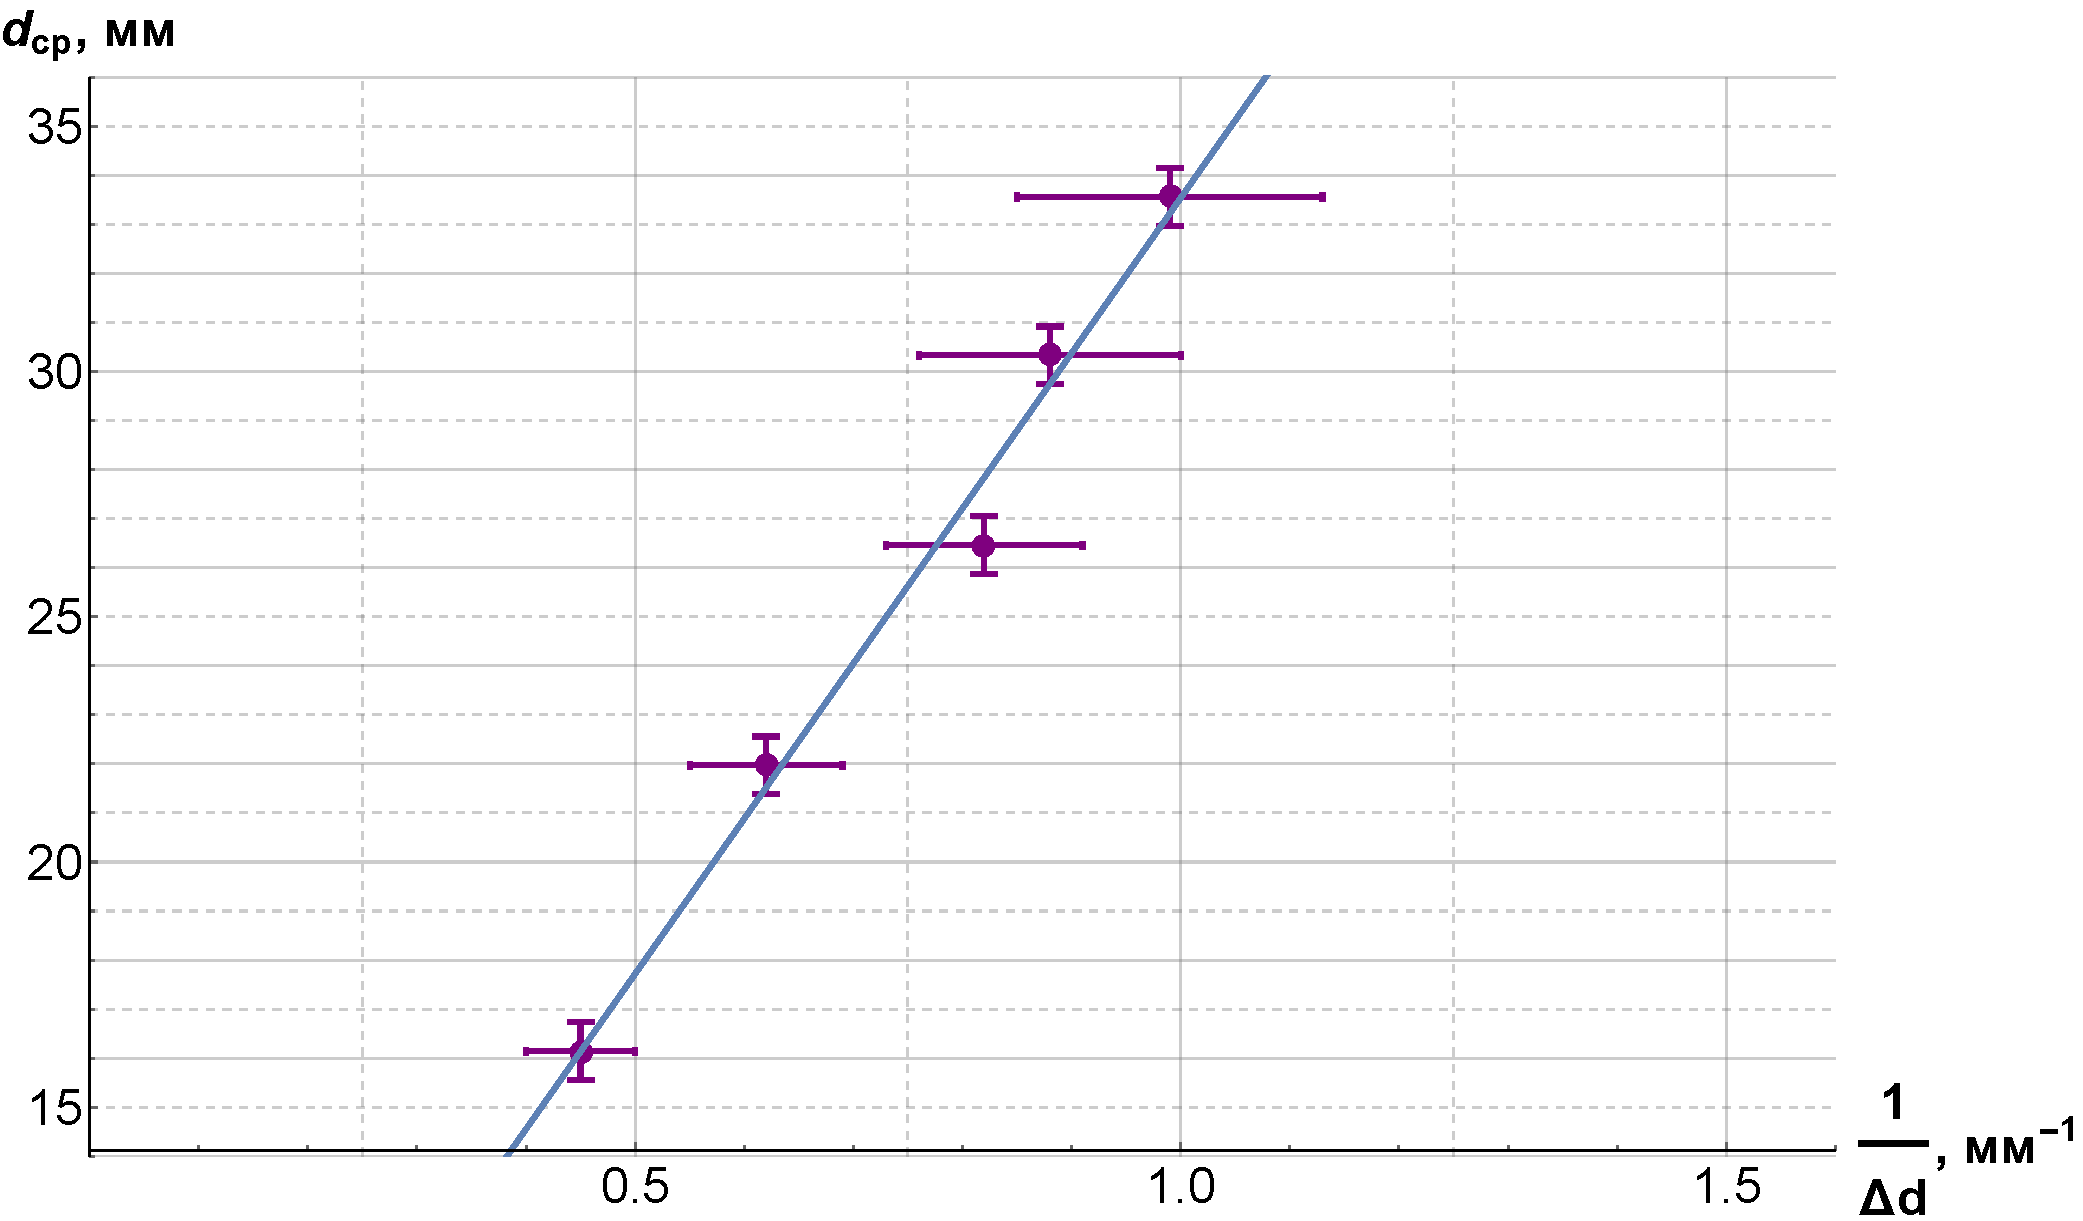
\includegraphics[scale=0.47]{na2.pdf}
		\caption{График зависимости $ \overline{d} $ от $ \dfrac{1}{\Delta d}$ линий $ Na $}
	\end{figure}
	
	\begin{table}[h]
		\centering
		\caption{Расчет апроксимированной прямой $ y = ax +b $}
		\begin{tabular}{c|cc}
			\text{} & \text{Estimate} & \text{Standard Error} \\
			\hline
			a & 
			33,6 & 2,1
			\\
			b & 1,8 & 0,7  \\
		\end{tabular}
	\end{table}

	Из полученных данных $ a = \overline{d} \Delta d = (33,6 \pm 2,1) \x 10^{-6} м^2 $ рассчитаем разность длин волн $ \Delta \lambda_р  $ интерферометра, взяв $ \lambda(Hg) =  5893 $ \AA :

	\begin{equation}\label{}
	\Delta \lambda_р = \dfrac{\lambda a}{4f^2} = (5,6 \pm 0,4) \text{\AA}
	\end{equation}
	
	\subsection{Дополнительные расчеты}
	
	Сравним теоретические и экспериментальные значения линейной дисперсии интерферометра:
	
	\begin{table}[]
		\caption{Сравнение линейной дисперсии}
		\begin{center}
			\begin{tabular}{|c|c|c|c|c|c|c|c|c|}
				\hline
				$ \Delta d $, мм & $ D_э $, мм/\AA & 	$ \overline{d} $, мм & $ D_т $, мм/\AA  & $ <- Hg \; \; Na ->	 $&$ \Delta d $, мм & $ D_э $, мм/\AA & 	$ \overline{d} $, мм & $ D_т $, мм/\AA     \\
				\hline
			3.12 & 0.39 & 15.78 & 0.27 & & 2.22 & 0.2 & 16.14 & 0.19 \\
			1.97 & 0.25 & 22.32 & 0.19 & & 1.61 & 0.14 & 21.97 & 0.14 \\
			1.68 & 0.21 & 27.15 & 0.15 & & 1.22 & 0.11 & 26.46 & 0.11 \\
			1.35 & 0.17 & 30.96 & 0.14 & &1.13 & 0.1 & 30.33 & 0.1 \\
			1.11 & 0.14 & 34.6 & 0.12 & &1.01 & 0.09 & 33.56 & 0.09 \\
				\hline
			\end{tabular}
		\end{center}
		\label{}
	\end{table}

	Расчеты по формуле:
	
	\begin{equation}\label{}
	D_э = \dfrac{\Delta d}{2 \Delta \lambda}, \quad D_т = \dfrac{2f^2}{\lambda \overline{d}}
	\end{equation}
	
	Рассчитаем аппаратную разрешающую способность:
	
	\begin{equation}\label{}
	R_а = \dfrac{\lambda}{\delta \lambda} \backsimeq \dfrac{4f^2}{d \delta r}
	\end{equation}
	
	Для ртути $ R_a = 5,5 \x 10^{-3} $, для натрия $ R_a = 7,1 \x 10^{-3} $.
	
	

	
\end{document}